\scanpage{41}
\figure{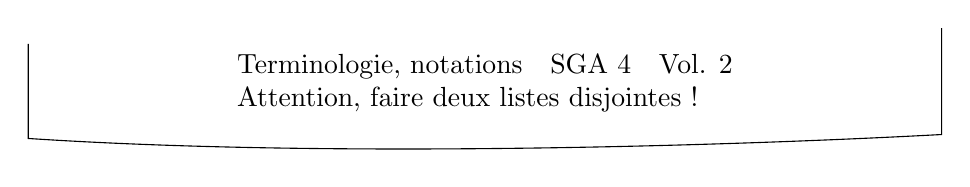
\begin{tikzpicture}
\node[align=left] at (0,0) {\handwritten{Terminologie, notations\quad SGA 4\quad Vol. 2}\\\handwritten{Attention, faire \uline{deux} listes disjointes !}};
\draw (-5.8,.5)--(-5.8,-.7) .. controls (-2,-.95) and (3,-.8) .. (5.8,-.65)--(5.8,.7);
\end{tikzpicture}}

\figure{\begin{tikzpicture}
\node[align=left] at (0,0) {(Sch)\qquad VII 1.1\\$\operatorname{Et}_{/X}\handwritten{,}\ X_{\mathrm{ét}}$\quad VII 1.2};
\draw (0,0) ellipse (2.8cm and .8cm);
\end{tikzpicture}}

Topologie étale (sur (Sch), sur un schéma)\quad étale topology (on (Sch), \inserted{on a scheme)}\handwritten{)}\quad VII 1.2

site étale d'un schéma\quad étale site of a scheme\quad VII 1.2

topos étale d'un schéma\quad étale topos of a scheme\quad VII 1.2

\figure{\begin{tikzpicture}
\node at (0,0) {$f_{\mathrm{ét}}$\qquad VII \unsure{1.4|1.1.4}};
\draw[line width=.8pt] (.65,.08)--(.78,.30);
\draw (0,0) ellipse (2.6cm and .4cm);
\end{tikzpicture}}
% A handwritten dark correction overlaps the middle of the f_et reference.

point géométrique d'un schéma\quad geometric point of a scheme\quad VIII 3.1.

foncteur fibre (relatif à un point géométrique d'un schéma)\quad fiber functor\deleted{\unsure{s}} (corresponding to a geometric point of a scheme)\quad VIII 3.3

\figure{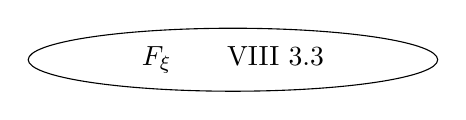
\begin{tikzpicture}
\node at (0,0) {$F_{\handwritten{\xi}}$\qquad VIII 3.3};
\draw (0,0) ellipse (2.6cm and .4cm);
\end{tikzpicture}}

hensélien (anneau local - )\quad henselian local ring\quad VIII 4.1

\deleted{Clôture} \unsure{hensélisé}\deleted{\unsure{enne|en}} d'un anneau local\quad henselization of a local ring\quad VIII 4.1

strictement local (anneau)\quad strictly local ring\quad VIII 4.2

\handwritten{---} id \handwritten{---} (schéma)\quad strictly local scheme\quad VIII 4.2

anneau \deleted{\unsure{à}}strictement local (d'un schéma en un point géométrique)\quad strictly local ring (of a scheme \unsure{àt|at} a geometric point)\quad VIII 4.3

hensélisé strict d'un anneau local\quad strict hens\deleted{\unsure{\'{}}}elisation of a local ring\quad VIII 4.4

localisé strict d'un schéma en un point géométrique\quad strict localization of a scheme at a geometric point\quad VIII 4.3

flèche de spécialisation\quad speciali\deleted{\unsure{s}}zation \deleted{\unsure{morphism}}\inserted{arrow}\quad VIII 7.2

spécialisation d'un point géométrique\quad specialization of a geometric \unsure{point}\quad VIII 7.2

générisation d'un point géométrique\quad generization of a geometric point\quad VIII 7.2

\figure{\begin{tikzpicture}
\node at (0,0) {$\handwritten{\overline}{X}(\handwritten{\xi})$};
\draw[rotate=35] (0,0) ellipse (.65cm and .4cm);
\node[anchor=west] at (.8,0) {($\handwritten{\xi}$ point géométrique du schéma $X$)\quad VIII 7.1};
\end{tikzpicture}}

Homomorphisme de spécialisation\quad \deleted{\unsure{f|t}} specialization homomorphism\quad VIII 7.7

\figure{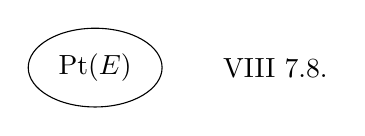
\begin{tikzpicture}
\node at (0,0) {\uline{Pt}$(E)$};
\draw (0,0) ellipse (.85cm and .5cm);
\node[anchor=west] at (1.5,0) {VIII 7.8.};
\end{tikzpicture}}
% archive sheet number: 40
